%! TeX root = 9.2exercise.tex
\documentclass[12pt, a4paper]{article}

% Required Packages
\usepackage{amsmath, amssymb, graphicx}
\usepackage{kotex} % For Korean text
\usepackage{geometry}
\graphicspath{{graph/}}
\geometry{a4paper, margin=1in}
\title{Calculus - Chapter 9.2 Exercises}
\begin{document}
\maketitle

\subsection*{난이도 하}
\begin{enumerate}
    \item \textbf{Exercise 1(a):} A direction field for the differential equation $y' = x \cos(\pi y)$ is shown. Sketch the graphs of the solutions that satisfy the given initial conditions.
    \begin{itemize}
        \item[(i)] $y(0)=0$
        \item[(ii)] $y(0)=0.5$
    \end{itemize}
    
    \begin{figure}[htbp] % [h!] 옵션은 여기에(here!) 그림을 위치시키라는 의미
         \centering % 이미지를 가운데로 정렬
        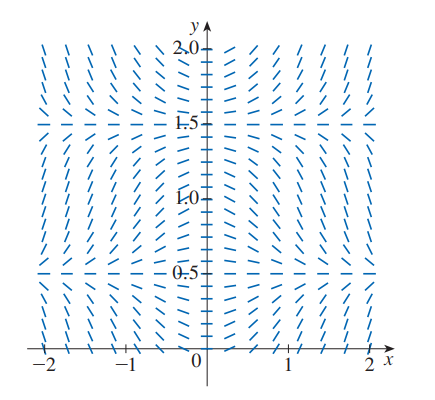
\includegraphics[width=0.3\textwidth]{graph1.png} % 너비는 텍스트 너비의 70%    
    \end{figure}

    \item \textbf{Exercise 1(b):} Find all the equilibrium solutions for the differential equation in Exercise 1.

    \item \textbf{Exercise 21:} Use Euler's method with step size 0.5 to compute the approximate y-values $y_1, y_2, y_3,$ and $y_4$ of the solution of the initial-value problem $y' = y - 2x$, $y(1)=0$.

    \item \textbf{Exercise 23:} Use Euler's method with step size 0.1 to estimate $y(0.5)$, where $y(x)$ is the solution of the initial-value problem $y' = y + xy, y(0)=1$.
\end{enumerate}

\hrulefill
\vspace{1em}

\subsection*{난이도 중 }
\begin{enumerate}
    \setcounter{enumi}{4} % Continue numbering
    \item \textbf{Exercise 3:} Match the differential equation $y' = 2 - y$ with its direction field (labeled I-IV). Give reasons for your answer.
    
     \begin{figure}[htbp]
        \centering
        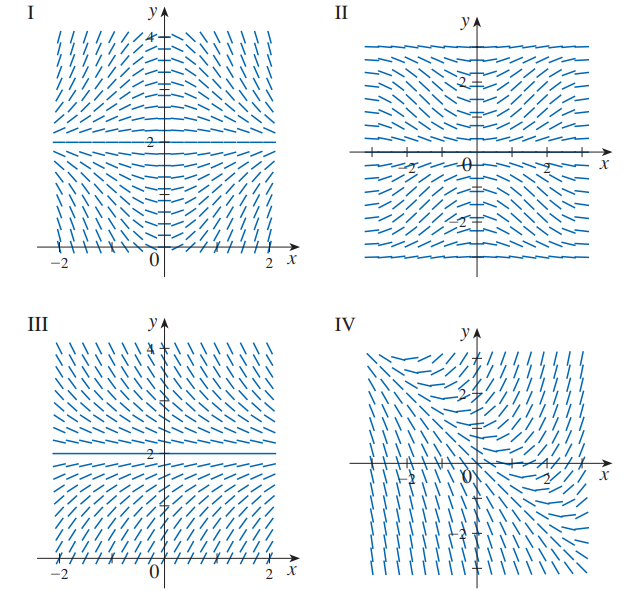
\includegraphics[width=0.5\textwidth]{graph2.png} % 너비는 텍스트 너비의 80%
    \end{figure}


    \item \textbf{Exercise 4:} Match the differential equation $y' = x(2 - y)$ with its direction field (labeled I-IV). Give reasons for your answer.

    \item \textbf{Exercise 9:} Sketch a direction field for the differential equation $y' = \frac{1}{2}y$. Then use it to sketch three solution curves.

    \item \textbf{Exercise 11:} Sketch the direction field of the differential equation $y' = y - 2x$. Then use it to sketch a solution curve that passes through the point $(1,0)$.

    \item \textbf{Exercise 19(a):} Use Euler's method with step size $h=0.1$ to estimate the value of $y(0.4)$ where $y$ is the solution of the initial-value problem $y' = y, y(0)=1$.

    \item \textbf{Exercise 19(c):} The error in Euler's method is the difference between the exact value and the approximate value. Find the errors made in part (a) in using Euler's method to estimate the true value of $y(0.4)$, namely, $e^{0.4}$.

    \item \textbf{Exercise 20:} A direction field for a differential equation is shown. Draw, with a ruler, the graphs of the Euler approximations to the solution curve that passes through the origin. Use step sizes $h=1$ and $h=0.5$. Will the Euler estimates be underestimates or overestimates? Explain.
    
    \begin{center}
        \begin{figure}[htbp] % [h!] 옵션은 여기에(here!) 그림을 위치시키라는 의미
            \centering % 이미지를 가운데로 정렬
             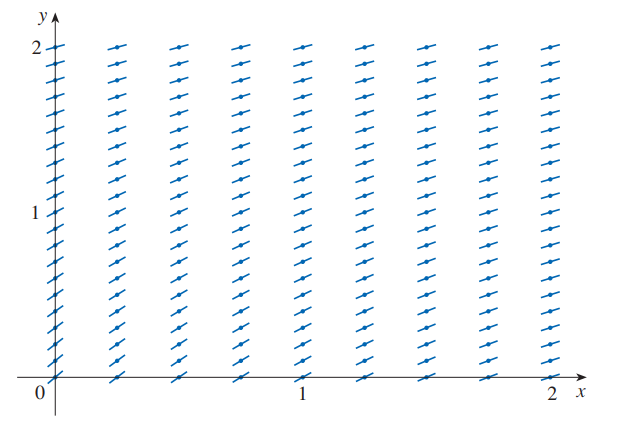
\includegraphics[width=0.5\textwidth]{graph3.png} % 너비는 텍스트 너비의 70%    
         \end{figure}
    \end{center}
\end{enumerate}

\hrulefill
\vspace{1em}

\subsection*{난이도 상}
\begin{enumerate}
    \setcounter{enumi}{11} % Continue numbering
    \item \textbf{Exercise 18:} Make a rough sketch of a direction field for the autonomous differential equation $y' = f(y)$, where the graph of f is as shown. How does the limiting behavior of solutions depend on the value of $y(0)$?
    
    \begin{center}
        \begin{figure}[htbp] % [h!] 옵션은 여기에(here!) 그림을 위치시키라는 의미
            \centering % 이미지를 가운데로 정렬
             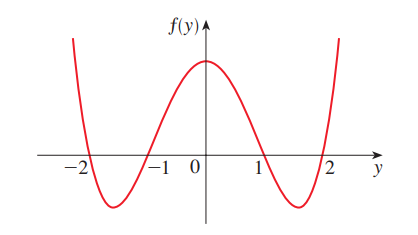
\includegraphics[width=0.4\textwidth]{graph4.png} % 너비는 텍스트 너비의 70%    
         \end{figure}
    \end{center}

    \item \textbf{Exercise 27(a):} For the given RC circuit, draw a direction field for the differential equation $R\frac{dQ}{dt}+\frac{1}{C}Q=E(t)$ with R=5$\Omega$, C=0.05F, and E(t)=60V.

    \item \textbf{Exercise 27(b, d):} Based on the direction field from part (a):
    \begin{itemize}
        \item[(b)] What is the limiting value of the charge?
        \item[(d)] If the initial charge is $Q(0)=0$ C, use the direction field to sketch the solution curve.
    \end{itemize}

    \item \textbf{Exercise 28(c):} For the cooling coffee problem modeled by a differential equation, use Euler's method with step size $h=2$ minutes to estimate the temperature of the coffee after 10 minutes.
\end{enumerate}

\end{document}
